\documentclass[14pt, a4paper]{extarticle}
\usepackage{mospolytech_coursework}
\usepackage{float}
\usepackage{makecell}

% Определение данных
\newcommand{\theme}{%
    Разработка веб-приложения для управления и мониторинга CI/CD-пайплайнов%
}
\newcommand{\subject}{Разработка веб-приложений}
\newcommand{\student}{Мижитдоржиев Гэлэг Намдакович}
\newcommand{\group}{241-327}
\newcommand{\teacher}{Кружалов Алексей Сергеевич}

\begin{document}

% Титульный лист
\include{title}

% Задание
% После сборки task.tex в task.pdf можно раскомментировать строку ниже.
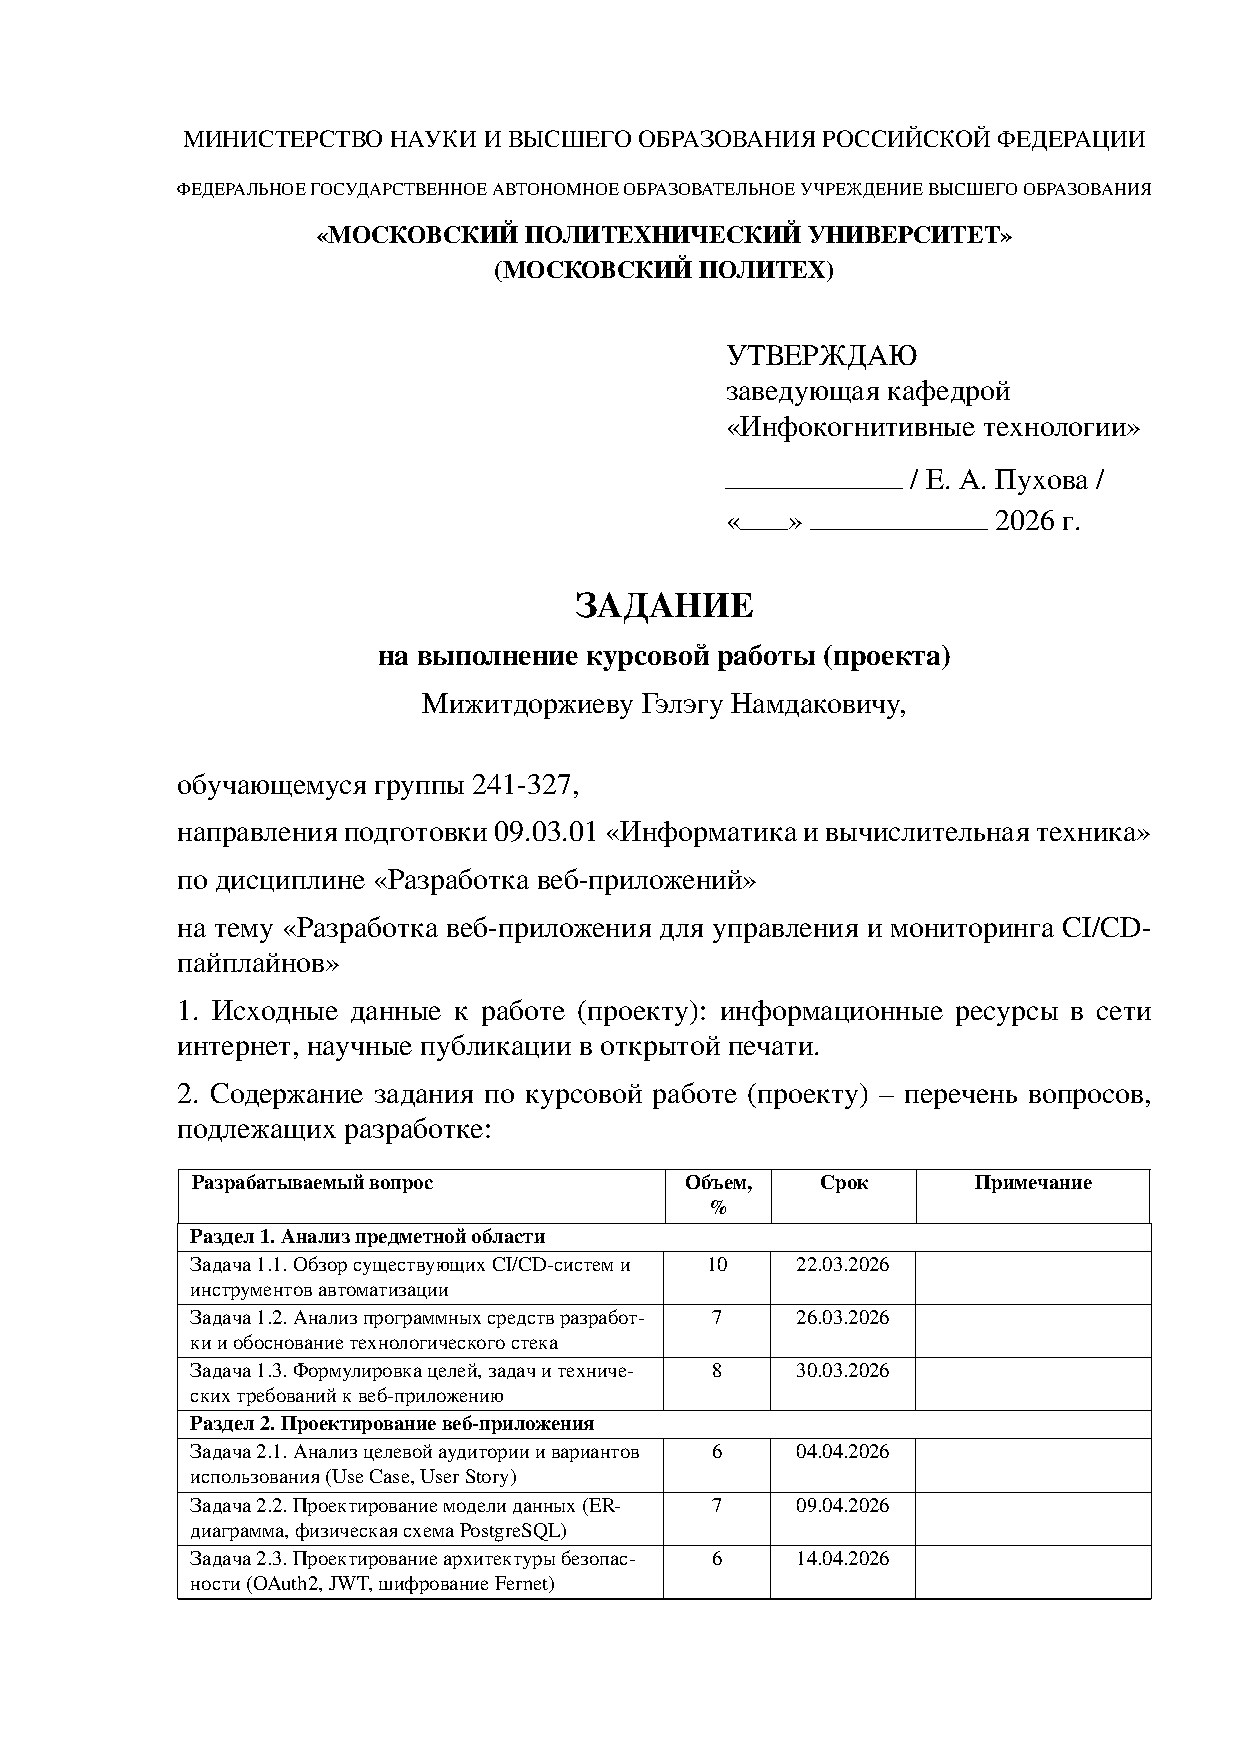
\includepdf[pages=-]{task.pdf}

% Содержание
\tableofcontents

% Введение
\section*{Введение}
\addcontentsline{toc}{section}{Введение}

В современных условиях разработка программного обеспечения требует высокой скорости выпуска обновлений и постоянного контроля качества. Для решения этих задач команды используют практики непрерывной интеграции и непрерывной доставки, позволяющие автоматически запускать сборку, тестирование и развертывание приложений после изменений в исходном коде.

При росте количества проектов, окружений и команд CI/CD-процессы становятся сложнее. Информация о пайплайнах может находиться в разных системах: GitHub Actions, GitLab CI/CD, Jenkins, Argo CD и других инструментах. Разработчикам и DevOps-инженерам приходится переключаться между несколькими интерфейсами, вручную отслеживать статусы запусков, искать причины ошибок в логах и контролировать готовность релизов. Это увеличивает время реакции на сбои и снижает прозрачность процесса разработки.

Актуальность темы обусловлена необходимостью создания единого веб-интерфейса, который позволит централизованно управлять CI/CD-пайплайнами и отслеживать их состояние. Такое приложение может использоваться для просмотра проектов, запусков, этапов выполнения, логов, истории статусов и результатов сборки. Наличие единой панели мониторинга упрощает контроль качества и помогает быстрее выявлять проблемные участки процесса поставки программного обеспечения.

Цель курсового проекта --- разработать веб-приложение для управления и мониторинга CI/CD-пайплайнов.

Для достижения цели необходимо решить следующие задачи:
\begin{itemize}
    \item проанализировать предметную область и существующие CI/CD-инструменты;
    \item выбрать программные средства разработки и технологический стек;
    \item сформулировать требования к веб-приложению;
    \item спроектировать структуру приложения и модель данных;
    \item реализовать основные функции управления проектами, пайплайнами, запуском и просмотром логов;
    \item провести проверку работоспособности основных сценариев.
\end{itemize}

Объектом исследования являются процессы автоматизации сборки, тестирования и развертывания программного обеспечения. Предметом исследования является веб-приложение, обеспечивающее управление и мониторинг CI/CD-пайплайнов.

Курсовой проект состоит из введения, аналитического раздела, разделов проектирования и реализации, заключения и списка использованных источников. В первом разделе рассматриваются существующие CI/CD-системы, проводится выбор технологического стека и формулируются требования к разрабатываемому приложению.


% Основная часть
\section*{Глава 1. Анализ предметной области}
\addcontentsline{toc}{section}{Глава 1. Анализ предметной области}
\stepcounter{section}

\subsection{Обзор существующих CI/CD-систем и инструментов автоматизации}

Современная разработка программного обеспечения все чаще строится вокруг практик непрерывной интеграции и непрерывной доставки (CI/CD). CI/CD-пайплайн представляет собой формализованную последовательность этапов, в которой исходный код автоматически проверяется, собирается, тестируется и подготавливается к развертыванию. Такой подход снижает количество ручных операций, ускоряет выпуск новых версий и делает процесс поставки программного продукта более прозрачным и контролируемым.

Для инженерных команд критически важны не только внутренние механизмы исполнения сборок, но и удобные средства мониторинга и оперативного управления: централизованное отображение текущих запусков, контроль сбоев, анализ логов, возможность ручного перезапуска упавших задач и оценка стабильности процессов. При использовании микросервисной архитектуры и распределении сервисов по десяткам репозиториев стандартные интерфейсы отдельных CI/CD-систем приводят к фрагментации контроля. Возникает потребность в специализированном веб-приложении, агрегирующем данные из внешних сервисов автоматизации в концепции единого окна («Single Pane of Glass»).

В рамках анализа предметной области рассмотрены наиболее распространенные решения: GitHub Actions, GitLab CI/CD, Jenkins и Argo CD.

\textbf{GitHub Actions} --- встроенная в платформу GitHub система автоматизации, в которой сценарии описываются в виде workflow-файлов формата YAML. Система глубоко интегрирована с событиями репозитория: pull requests, коммитами, релизами и внутренним хранилищем секретов. Данное решение оптимально для проектов, размещенных на GitHub~\cite{github_actions_docs}. Однако его ключевым ограничением является жесткая привязка к экосистеме GitHub, что затрудняет сквозной мониторинг гетерогенной инфраструктуры.

\textbf{GitLab CI/CD} --- компонент комплексной DevOps-платформы GitLab, конфигурируемый через файл \texttt{.gitlab-ci.yml}. Решение предоставляет развитые возможности по управлению стадиями, зависимостями задач, собственными runner-агентами, переменными окружения и артефактами~\cite{gitlab_cicd_docs}. Главным достоинством является полнота экосистемы, а ограничением --- ориентация на закрытый контур GitLab, требующая отдельной настройки внешних интеграций через REST API и webhooks.

\textbf{Jenkins} --- классическая расширяемая система автоматизации с открытым исходным кодом. Механизм Jenkins Pipeline позволяет описывать сложные сценарии сборки в файлах Jenkinsfile~\cite{jenkins_pipeline_docs}. Система независима от Git-хостинга и обладает обширной экосистемой плагинов. К ее недостаткам относятся высокая ресурсоемкость, сложность администрирования и визуальная неоднородность интерфейса.

\textbf{Argo CD} --- декларативный инструмент GitOps-доставки приложений в среду Kubernetes. Argo CD отслеживает состояние манифестов в Git-репозитории и синхронизирует их с фактическим состоянием кластера~\cite{argo_cd_docs}. Данный инструмент не предназначен для выполнения этапов компиляции и тестирования, а используется на финальной стадии доставки совместно с традиционными CI-системами.

Сравнительная характеристика рассмотренных инструментов автоматизации приведена в таблице~\ref{tab:cicd_compare}.

\begin{table}[H]
    \centering
    \caption{Сравнительный анализ CI/CD-систем}
    \label{tab:cicd_compare}
    \small
    \begin{tabular}{|p{2.4cm}|p{3.1cm}|p{3.1cm}|p{3.2cm}|p{3.2cm}|}
        \hline
        \textbf{Система} & \textbf{Основное назначение} & \textbf{Сильные стороны} & \textbf{Ограничения} & \textbf{Значимость для проекта} \\ \hline
        GitHub Actions & Автоматизация workflow внутри GitHub & Простая настройка, развитая экосистема actions, тесная связь с PR & Привязка к GitHub, лимиты бесплатного времени runner & Источник данных для интеграции через GitHub REST API \\ \hline
        GitLab CI/CD & Полный цикл CI/CD в среде GitLab & Единая платформа, runner-агенты, артефакты, environments & Зависимость от инфраструктуры GitLab & Источник данных для интеграции через GitLab API \\ \hline
        Jenkins & Универсальная система автоматизации & Предельная гибкость, независимость от хостинга кода & Сложность поддержки, устаревший базовый интерфейс & Потенциальный источник интеграции внешних jobs \\ \hline
        Argo CD & GitOps-доставка в Kubernetes & Синхронизация состояний, надежный деплой в кластер & Не выполняет этапы сборки и модульного тестирования & Пример специализированного инструмента доставки \\ \hline
    \end{tabular}
\end{table}

Проведенный анализ показывает, что инструменты CI/CD эффективно функционируют внутри своих экосистем, однако в командах с гетерогенной инфраструктурой инженерам приходится постоянно переключаться между различными панелями управления. 

Разрабатываемое веб-приложение призвано решить эту проблему в роли централизованного агрегатора и пульта управления: оно должно собирать актуальные статусы сборок через API внешних систем, хранить историю запусков, предоставлять быстрый доступ к логам и поддерживать диспетчеризацию (повторный запуск упавших пайплайнов) из единого интерфейса.

\subsection{Анализ программных средств разработки и выбор технологического стека}

Для реализации веб-приложения мониторинга и диспетчеризации пайплайнов необходим технологический стек, обеспечивающий высокую отзывчивость интерфейса, эффективную асинхронную обработку внешних сетевых запросов и безопасное хранение учетных записей и токенов интеграций.

Архитектура системы строится на разделении клиентской части (Single Page Application, SPA) и серверной части (REST API), взаимодействующих по протоколам HTTP/JSON и WebSocket.

\textbf{Клиентская часть.} Интерфейс системы мониторинга должен в реальном времени отображать статусы большого количества параллельных процессов, предоставлять средства динамической фильтрации, поиска по веткам и коммитам, а также отрисовывать графики стабильности сборок. Для разработки клиентского приложения рассмотрены технологии React, Vue.js и серверная генерация HTML (Jinja/Blade).

\begin{table}[H]
    \centering
    \caption{Сравнение фронтенд-технологий}
    \label{tab:frontend_compare}
    \small
    \begin{tabular}{|p{3cm}|p{3.7cm}|p{3.7cm}|p{3.7cm}|}
        \hline
        \textbf{Критерий} & \textbf{React (выбран)} & \textbf{Vue.js} & \textbf{Jinja (серверный рендеринг)} \\ \hline
        Архитектурный подход & SPA на базе компонентов и Virtual DOM~\cite{react_docs} & SPA на базе реактивных компонентов & Серверная генерация статических страниц \\ \hline
        Динамичность интерфейса & Мгновенное обновление карточек статусов без перезагрузки & Быстрое реактивное обновление DOM-дерева & Требует полной перезагрузки страницы или сложных скриптов \\ \hline
        Экосистема для дашбордов & Огромный выбор библиотек (Lucide, Recharts, Tailwind UI) & Достаточный выбор библиотек компонентов & Ограничена базовыми CSS-фреймворками \\ \hline
        Разделение ответственности & Полная изоляция логики представления от бэкенда & Полная изоляция клиентской части & Жесткая связность с кодом серверного фреймворка \\ \hline
    \end{tabular}
\end{table}

В качестве основы фронтенда выбрана библиотека \textbf{React}. Компонентный подход позволяет изолировать логику отображения отдельных карточек пайплайнов, индикаторов статусов и модальных окон управления. Использование Virtual DOM и хуков состояния обеспечивает высокую производительность при частых обновлениях данных через WebSockets без необходимости перерисовки всего экрана. Сборка проекта осуществляется с использованием современного инструмента Vite.

\textbf{Серверная часть.} Сервер приложения выполняет функции шлюза и агрегатора: принимает HTTP-запросы от клиентской части, осуществляет фоновый опрос и прием webhooks от внешних платформ (GitHub Actions, GitLab CI/CD), сохраняет промежуточные снапшоты в БД и транслирует команды повторного запуска (re-run). Для серверной реализации рассмотрены фреймворки на языке Python: FastAPI, Flask и Django.

\begin{itemize}
    \item \textbf{FastAPI (выбран)}: современный высокопроизводительный асинхронный фреймворк, построенный на базе ASGI-сервера Starlette и библиотеки валидации данных Pydantic~\cite{fastapi_docs}. Ключевым преимуществом FastAPI является нативная поддержка корутин (\texttt{async/await}), что критически важно для приложения-агрегатора, совершающего множество параллельных сетевых I/O-запросов к внешним API без блокировки основного потока. Кроме того, фреймворк автоматически генерирует интерактивную OpenAPI-документацию (Swagger UI).
    \item \textbf{Flask}: классический микрофреймворк с синхронной архитектурой (WSGI). Реализация высоконагруженного асинхронного взаимодействия с внешними API и работа с протоколом WebSocket во Flask требуют подключения дополнительных надстроек, что усложняет архитектуру.
    \item \textbf{Django}: полнофункциональный монолитный фреймворк. Включает избыточный для компактного API-сервиса функционал (административную панель, встроенный ORM с привязкой к синхронным вызовам), что создает лишние накладные расходы при разработке легковесного шлюза.
\end{itemize}

С учетом необходимости асинхронного ввода-вывода и строгой типизации контрактов API в качестве серверного фреймворка выбран \textbf{FastAPI}.

\textbf{Хранение данных.} Для долговременного хранения сведений о зарегистрированных пользователях, проектах, конфигурациях токенов доступа и исторических метрик сборок выбрана реляционная СУБД \textbf{PostgreSQL}~\cite{postgresql_docs}. Наличие поддержки типа данных \texttt{JSONB} позволяет сохранять неструктурированные метаданные внешних webhooks без усложнения реляционной схемы. Для взаимодействия с базой данных используется асинхронная ORM SQLAlchemy~2.0 в связке с драйвером \texttt{asyncpg}, а миграции схемы выполняются с помощью инструмента Alembic.

\textbf{Взаимодействие компонентов и внешняя интеграция.} Связь между SPA-клиентом и бэкендом организуется через REST API в формате JSON, а для моментальной доставки сведений об изменении статуса пайплайна используются протокол WebSocket и механизм Webhooks. Сетевые запросы к API внешних провайдеров (GitHub REST API v3, GitLab REST API v4) осуществляются с использованием асинхронного HTTP-клиента \texttt{httpx}.

Сводная информация о выбранном стеке приведена в таблице~\ref{tab:stack}.

\begin{table}[H]
    \centering
    \caption{Выбранный технологический стек}
    \label{tab:stack}
    \small
    \begin{tabular}{|p{4cm}|p{4.6cm}|p{5.2cm}|}
        \hline
        \textbf{Компонент} & \textbf{Выбранная технология} & \textbf{Назначение} \\ \hline
        Клиентская часть & React, TypeScript, Vite & Интерактивный SPA-интерфейс дашборда, карточки пайплайнов, графики \\ \hline
        Серверная часть & Python, FastAPI & Асинхронный REST API, диспетчеризация задач, валидация данных через Pydantic \\ \hline
        База данных & PostgreSQL & Надежное хранение проектов, пользователей, токенов и истории запусков \\ \hline
        ORM и миграции & SQLAlchemy 2.0 (async), Alembic & Управление реляционной схемой и асинхронный доступ к БД \\ \hline
        Обмен данными & REST API, Webhooks, WebSocket & Взаимодействие с клиентом и интеграция с внешними CI/CD-платформами \\ \hline
        Развертывание & Docker, Docker Compose & Контейнеризация сервисов и изоляция тестового окружения \\ \hline
    \end{tabular}
\end{table}

Выбранная архитектура на базе FastAPI и React разделяет ответственность между представлением и бизнес-логикой, гарантирует высокую скорость отклика и позволяет гибко подключать новых CI/CD-провайдеров.

\subsection{Формулировка цели, задач и требований проекта}

Основная инженерная проблема заключается в фрагментации данных о сборках при одновременной разработке множества микросервисов в разных системах контроля версий. Разрабатываемое веб-приложение призвано стать единой точкой наблюдения и диспетчеризации.

\textbf{Цель работы} --- разработать веб-приложение для централизованного управления и мониторинга CI/CD-пайплайнов, агрегирующее статусы сборок из внешних систем автоматизации и предоставляющее пользователю интерфейс оперативного реагирования и аналитики.

Для достижения поставленной цели необходимо решить следующие \textbf{задачи}:
\begin{enumerate}
    \item Провести анализ существующих платформ CI/CD и выявить ключевые функциональные требования к централизованной панели мониторинга.
    \item Обосновать выбор технологического стека для реализации SPA-клиента, асинхронного серверного API и хранилища данных.
    \item Спроектировать архитектуру веб-приложения и реляционную модель базы данных с учетом поддержки гетерогенных внешних источников.
    \item Реализовать модуль аутентификации пользователей и безопасного хранения токенов доступа к внешним сервисам.
    \item Разработать программные адаптеры для интеграции с внешними API (GitHub Actions REST API, GitLab API).
    \item Реализовать пользовательский интерфейс дашборда на React, обеспечивающий фильтрацию сборок, отображение карточек состояния и запуск команд повторного прогона (re-run).
    \item Реализовать механизмы оперативного обновления информации (Webhooks и WebSockets).
    \item Выполнить функциональное тестирование системы и оценить корректность обработки сбоев внешних сервисов.
\end{enumerate}

К разрабатываемому приложению предъявляются следующие \textbf{функциональные требования}:
\begin{itemize}
    \item аутентификация и авторизация пользователей в системе;
    \item управление подключениями к внешним провайдерам (ввод и безопасное хранение персональных токенов доступа);
    \item добавление и группировка отслеживаемых репозиториев и конвейеров сборки;
    \item сбор и синхронизация статусов пайплайнов (Success, Failed, Running, Queued, Canceled);
    \item отображение детальной информации о прогоне (автор коммита, ветка, хеш коммита, время выполнения и шаги пайплайна);
    \item возможность инициирования повторного запуска пайплайна (Re-run / Retry) через внешний API непосредственно из веб-интерфейса;
    \item фильтрация и поиск пайплайнов по статусу, проекту, автору и ветке;
    \item расчет базовых показателей надежности процессов (процент успешных прогонов и динамика длительности сборки).
\end{itemize}

Также сформированы \textbf{нефункциональные требования}:
\begin{itemize}
    \item время отдачи кэшированных агрегированных данных клиентскому приложению --- не более 300~мс;
    \item асинхронная неблокирующая архитектура взаимодействия с внешними сервисами;
    \item шифрование конфиденциальных данных (токенов доступа) при сохранении в базе данных;
    \item документирование REST API посредством автоматически генерируемой спецификации OpenAPI;
    \item масштабируемость архитектуры: возможность добавления новых CI/CD-провайдеров путем реализации единого программного интерфейса адаптера;
    \item адаптивный дизайн клиентской части для комфортной работы на экранах с различным разрешением;
    \item поддержка контейнеризации всех сервисов с помощью Docker Compose для быстрого развертывания.
\end{itemize}

Сформулированные требования определяют вектор дальнейшего проектирования системы: разработку диаграмм вариантов использования, проектирование базы данных и разработку макетов интерфейса в следующих разделах работы.

\section*{Глава 2. Проектирование веб-приложения}
\addcontentsline{toc}{section}{Глава 2. Проектирование веб-приложения}
\stepcounter{section}

\subsection{Анализ целевой аудитории}

Эффективность проектирования веб-приложения для управления и мониторинга CI/CD-пайплайнов напрямую зависит от детального понимания потребностей будущих пользователей. В условиях командной разработки программного обеспечения с конвейерами непрерывной интеграции взаимодействуют специалисты с различными зонами ответственности.

На основе специфики предметной области выделены три ключевые группы пользователей:
\begin{enumerate}
    \item DevOps-инженеры и системные администраторы. Специалисты отвечают за стабильность сборочной инфраструктуры, конфигурацию раннеров и доступность внешних платформ. Их ключевой интерес заключается в сквозном контроле работоспособности конвейеров, обнаружении зависших задач, анализе времени прохождения стадий и устранении инфраструктурных сбоев.
    \item Разработчики программного обеспечения (Frontend, Backend, Fullstack). Основные потребители сервиса. Для них критически важно быстро получать обратную связь о статусе прохождения юнит-тестов, линтеров и сборок после отправки изменений в Git. В случае падения сборки разработчику необходим моментальный доступ к логам ошибки и возможность повторного перезапуска задачи в один клик.
    \item Технические руководители и тимлиды (Team Lead, Tech Lead). Пользователи заинтересованы в высокоуровневой аналитике: общем проценте успешных сборок (Success Rate), частоте релизов, выявлении нестабильных тестов и контроле готовности релизных веток.
\end{enumerate}

Для формализации требований сформированы репрезентативные профили целевых пользователей (User Personas), представленные в таблице~\ref{tab:user_personas}.

\begin{table}[H]
    \centering
    \caption{Профили целевых пользователей (User Personas)}
    \label{tab:user_personas}
    \small
    \resizebox{\textwidth}{!}{%
    \begin{tabular}{|p{3cm}|p{3.8cm}|p{4.2cm}|p{3.8cm}|}
        \hline
        \textbf{Персона} & \textbf{Контекст деятельности} & \textbf{Боли и проблемы} & \textbf{Ожидания от системы} \\ \hline
        Алексей, 28 лет, DevOps-инженер & Сопровождает 15 микросервисов, распределенных между GitHub и GitLab & Вынужден переключаться между десятком вкладок; сложно отслеживать зависшие сборки & Единая панель статусов; фильтрация по статусам; оперативные уведомления \\ \hline
        Илья, 23 года, Backend-разработчик & Пишет код, часто делает push в feature-ветки, ждет результатов тестов & Долго ищет упавший шаг в громоздких интерфейсах; сложный путь до кнопки «Retry» & Моментальное отображение статуса коммита; лог ошибки на одном экране; быстрый перезапуск \\ \hline
        Марина, 34 года, Team Lead & Контролирует поставку релизов и метрики качества в спринтах & Отсутствие наглядной сводки по стабильности репозиториев; разрозненные отчеты & Обзорный дашборд; графики успешности сборок; аналитика среднего времени прогона \\ \hline
    \end{tabular}%
    }
\end{table}

Проведенный анализ целевой аудитории показывает необходимость реализации гибкого интерфейса, предоставляющего как агрегированные сводные метрики для руководителей, так и детальные журналы сборок с кнопками управления для инженеров.

\subsection{Описание функциональности приложения}

Функциональная архитектура разрабатываемого приложения разделяется на модули управления учетными записями, конфигурации внешних интеграций, фонового сбора метрик и интерактивного взаимодействия с конвейерами.

\subsubsection{Диаграмма вариантов использования}

Для визуализации сценариев взаимодействия пользователей с системой построена диаграмма вариантов использования (Use Case diagram), представленная на рисунке~\ref{fig:use_case}.

\begin{figure}[H]
    \centering
    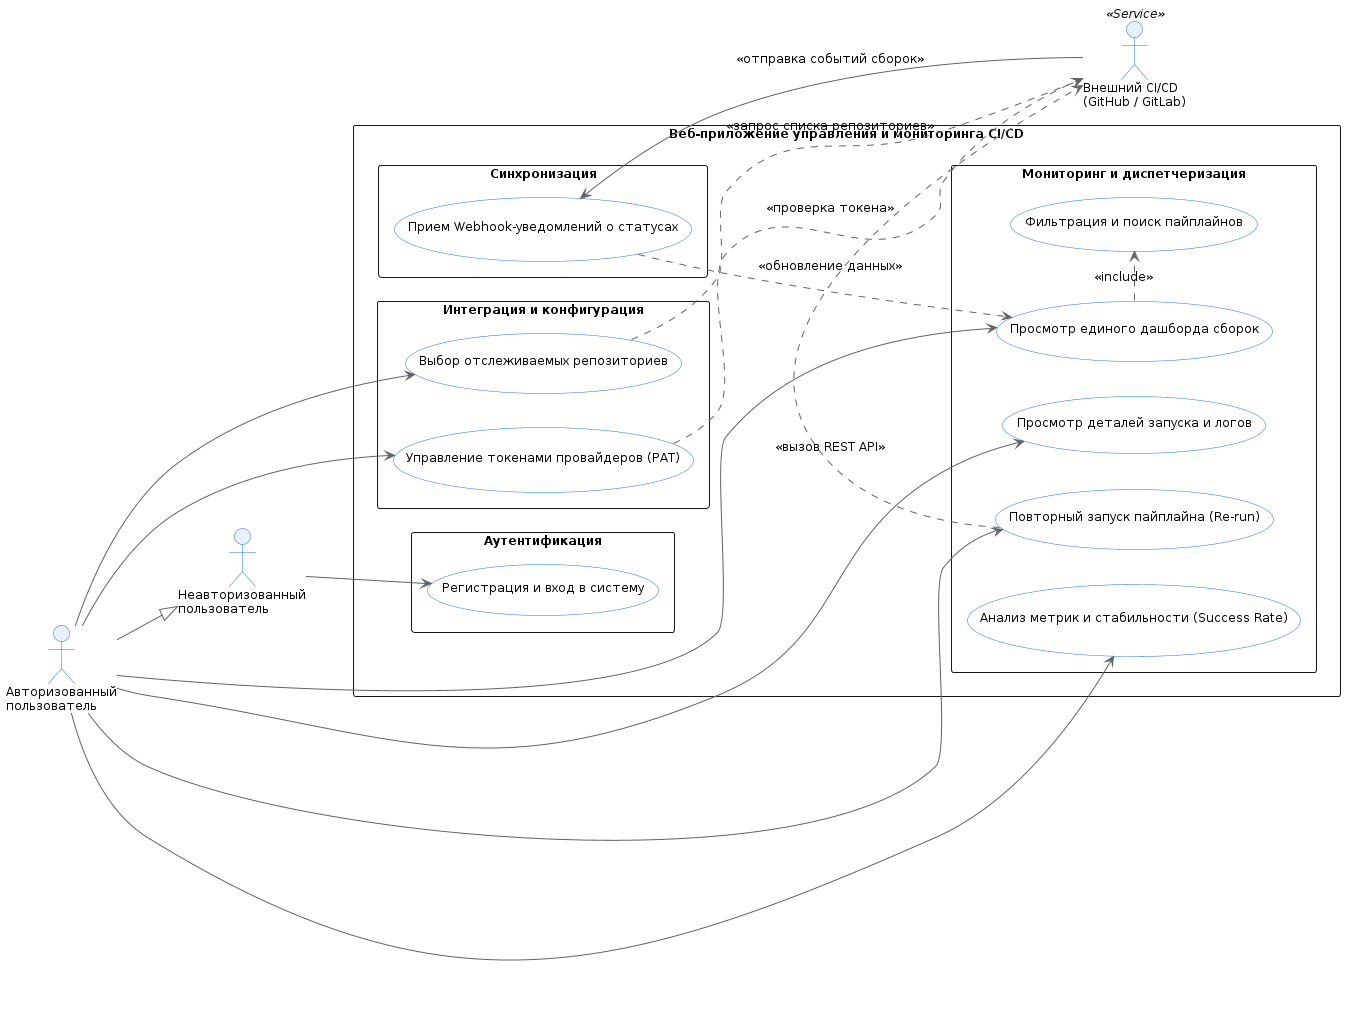
\includegraphics[width=0.85\textwidth]{images/use_case_diagram.png}
    \caption{Диаграмма вариантов использования веб-приложения}
    \label{fig:use_case}
\end{figure}

В системе выделены два действующих лица (актора):
\begin{itemize}
    \item неавторизованный пользователь (гость) --- имеет доступ только к формам входа и регистрации;
    \item авторизованный пользователь (инженер) --- имеет доступ к панели мониторинга, настройкам интеграций, управлению пайплайнами и аналитическим метрикам.
\end{itemize}

Ключевыми прецедентами являются:
\begin{itemize}
    \item управление токенами провайдеров CI/CD (GitHub PAT, GitLab Token);
    \item выбор и синхронизация отслеживаемых репозиториев;
    \item просмотр единого дашборда сборок;
    \item фильтрация и поиск пайплайнов по проектам, веткам и статусам;
    \item просмотр деталей запуска и логов выполнения сборок;
    \item диспетчеризация конвейера (повторный запуск упавших задач);
    \item анализ метрик надежности и стабильности сборок.
\end{itemize}

\subsubsection{Пользовательские истории (User Stories)}

Для детальной спецификации поведения системы разработаны пользовательские истории с критериями приемки (Acceptance Criteria), сведенные в таблицу~\ref{tab:user_stories}.

\begin{table}[H]
    \centering
    \caption{Пользовательские истории веб-приложения}
    \label{tab:user_stories}
    \small
    \resizebox{\textwidth}{!}{%
    \begin{tabular}{|l|p{4cm}|p{5cm}|p{5cm}|}
        \hline
        \textbf{ID} & \textbf{Пользовательская история} & \textbf{Критерии приемки (Given/When/Then)} & \textbf{Ценность для пользователя} \\ \hline
        US-01 & Как разработчик, я хочу подключить токен GitHub, чтобы отслеживать репозитории & \textbf{Given}: пользователь авторизован; \newline \textbf{When}: введен корректный PAT; \newline \textbf{Then}: токен зашифрован и сохранен & Безопасная интеграция без передачи основного пароля \\ \hline
        US-02 & Как инженер, я хочу видеть статусы сборок на одном экране, чтобы быстро выявлять сбои & \textbf{Given}: подключены провайдеры; \newline \textbf{When}: открыт дашборд; \newline \textbf{Then}: отображается таблица статусов & Экономия времени на переключение между системами \\ \hline
        US-03 & Как разработчик, я хочу перезапустить упавшую сборку в один клик, чтобы не заходить в GitHub & \textbf{Given}: сборка имеет статус Failed; \newline \textbf{When}: нажата кнопка «Retry»; \newline \textbf{Then}: статус сменился на Queued & Сокращение цикла исправления ошибок \\ \hline
        US-04 & Как тимлид, я хочу видеть процент успешности за неделю, чтобы оценить стабильность & \textbf{Given}: накоплена история запусков; \newline \textbf{When}: открыт раздел метрик; \newline \textbf{Then}: отображается Success Rate & Объективная оценка стабильности сборочных процессов \\ \hline
    \end{tabular}%
    }
\end{table}

\subsection{Проектирование модели данных}

Для обеспечения надежного хранения информации, транзакционной целостности и быстрого поиска по временным меткам выбрана реляционная модель данных, реализуемая в СУБД PostgreSQL.

\subsubsection{Концептуальная и логическая структура базы данных}

Модель данных спроектирована с учетом разделения сущностей на конфигурационные (пользователи, провайдеры, репозитории) и операционные (пайплайны, шаги выполнения, логи).

Связи между сущностями организованы следующим образом:
\begin{itemize}
    \item один пользователь (\texttt{users}) может сконфигурировать несколько подключений к внешним платформам (\texttt{ci\_providers}) --- связь «один-ко-многим» (1:N);
    \item каждый провайдер предоставляет доступ к множеству отслеживаемых репозиториев (\texttt{repositories}) --- связь «один-ко-многим» (1:N);
    \item репозиторий содержит историю запусков пайплайнов (\texttt{pipelines}) --- связь «один-ко-многим» (1:N);
    \item каждый запуск пайплайна детализируется последовательностью этапов выполнения (\texttt{pipeline\_steps}) --- связь «один-ко-многим» (1:N).
\end{itemize}

\subsubsection{Физическая схема базы данных}

Физическая схема разработана с соблюдением требований третьей нормальной формы (3NF). Для обеспечения информационной безопасности секретные ключи доступа (\texttt{encrypted\_token}) хранятся в зашифрованном виде с применением симметричного алгоритма Fernet.

Спецификация структуры таблиц приведена в таблицах~\ref{tab:table_users}--\ref{tab:table_steps}.

\begin{table}[H]
    \centering
    \caption{Спецификация таблицы пользователей (\texttt{users})}
    \label{tab:table_users}
    \small
    \resizebox{\textwidth}{!}{%
    \begin{tabular}{|l|l|l|p{7cm}|}
        \hline
        \textbf{Имя поля} & \textbf{Тип данных} & \textbf{Ключ} & \textbf{Описание и ограничения} \\ \hline
        \texttt{id} & INTEGER / SERIAL & PK & Уникальный идентификатор пользователя \\ \hline
        \texttt{email} & VARCHAR(255) & UNIQUE & Адрес электронной почты (логин), NOT NULL \\ \hline
        \texttt{hashed\_password} & VARCHAR(255) & — & Хеш пароля (алгоритм bcrypt), NOT NULL \\ \hline
        \texttt{full\_name} & VARCHAR(150) & — & Имя и фамилия пользователя \\ \hline
        \texttt{is\_active} & BOOLEAN & — & Флаг активности учетной записи (default: true) \\ \hline
        \texttt{created\_at} & TIMESTAMPTZ & — & Дата и время регистрации (default: NOW()) \\ \hline
    \end{tabular}%
    }
\end{table}

\begin{table}[H]
    \centering
    \caption{Спецификация таблицы провайдеров CI/CD (\texttt{ci\_providers})}
    \label{tab:table_providers}
    \small
    \resizebox{\textwidth}{!}{%
    \begin{tabular}{|l|l|l|p{7cm}|}
        \hline
        \textbf{Имя поля} & \textbf{Тип данных} & \textbf{Ключ} & \textbf{Описание и ограничения} \\ \hline
        \texttt{id} & INTEGER / SERIAL & PK & Идентификатор записи интеграции \\ \hline
        \texttt{user\_id} & INTEGER & FK & Внешний ключ на таблицу \texttt{users}, ON DELETE CASCADE \\ \hline
        \texttt{provider\_type} & VARCHAR(32) & — & Тип сервиса: \texttt{GITHUB}, \texttt{GITLAB} \\ \hline
        \texttt{name} & VARCHAR(100) & — & Пользовательское наименование подключения \\ \hline
        \texttt{api\_url} & VARCHAR(255) & — & Базовый URL API внешней платформы \\ \hline
        \texttt{encrypted\_token} & TEXT & — & Зашифрованный токен доступа (PAT), NOT NULL \\ \hline
        \texttt{is\_valid} & BOOLEAN & — & Статус валидности токена (default: true) \\ \hline
    \end{tabular}%
    }
\end{table}

\begin{table}[H]
    \centering
    \caption{Спецификация таблицы репозиториев (\texttt{repositories})}
    \label{tab:table_repos}
    \small
    \resizebox{\textwidth}{!}{%
    \begin{tabular}{|l|l|l|p{7cm}|}
        \hline
        \textbf{Имя поля} & \textbf{Тип данных} & \textbf{Ключ} & \textbf{Описание и ограничения} \\ \hline
        \texttt{id} & INTEGER / SERIAL & PK & Внутренний идентификатор репозитория \\ \hline
        \texttt{provider\_id} & INTEGER & FK & Внешний ключ на \texttt{ci\_providers}, ON DELETE CASCADE \\ \hline
        \texttt{external\_id} & VARCHAR(100) & — & Идентификатор проекта во внешней системе \\ \hline
        \texttt{full\_name} & VARCHAR(255) & — & Полное имя репозитория (\texttt{owner/repo}) \\ \hline
        \texttt{default\_branch} & VARCHAR(100) & — & Имя основной ветки (default: \texttt{main}) \\ \hline
        \texttt{web\_url} & VARCHAR(512) & — & Прямая веб-ссылка на репозиторий \\ \hline
        \texttt{is\_monitored} & BOOLEAN & — & Флаг активности мониторинга (default: true) \\ \hline
    \end{tabular}%
    }
\end{table}

\begin{table}[H]
    \centering
    \caption{Спецификация таблицы запусков пайплайнов (\texttt{pipelines})}
    \label{tab:table_pipelines}
    \small
    \resizebox{\textwidth}{!}{%
    \begin{tabular}{|l|l|l|p{7cm}|}
        \hline
        \textbf{Имя поля} & \textbf{Тип данных} & \textbf{Ключ} & \textbf{Описание и ограничения} \\ \hline
        \texttt{id} & INTEGER / SERIAL & PK & Внутренний идентификатор запуска \\ \hline
        \texttt{repository\_id} & INTEGER & FK & Внешний ключ на \texttt{repositories}, ON DELETE CASCADE \\ \hline
        \texttt{external\_run\_id} & VARCHAR(100) & — & Идентификатор прогона во внешнем API \\ \hline
        \texttt{branch} & VARCHAR(128) & — & Название целевой ветки коммита \\ \hline
        \texttt{commit\_sha} & VARCHAR(64) & — & Хеш-идентификатор коммита Git \\ \hline
        \texttt{commit\_message} & TEXT & — & Сообщение коммита \\ \hline
        \texttt{author\_name} & VARCHAR(150) & — & Автор изменений \\ \hline
        \texttt{status} & VARCHAR(32) & — & Статус: QUEUED, RUNNING, SUCCESS, FAILED \\ \hline
        \texttt{duration\_sec} & INTEGER & — & Длительность выполнения в секундах \\ \hline
        \texttt{started\_at} & TIMESTAMPTZ & — & Время запуска сборки \\ \hline
        \texttt{finished\_at} & TIMESTAMPTZ & — & Время завершения выполнения \\ \hline
    \end{tabular}%
    }
\end{table}

\begin{table}[H]
    \centering
    \caption{Спецификация таблицы стадий выполнения (\texttt{pipeline\_steps})}
    \label{tab:table_steps}
    \small
    \resizebox{\textwidth}{!}{%
    \begin{tabular}{|l|l|l|p{7cm}|}
        \hline
        \textbf{Имя поля} & \textbf{Тип данных} & \textbf{Ключ} & \textbf{Описание и ограничения} \\ \hline
        \texttt{id} & INTEGER / SERIAL & PK & Внутренний идентификатор шага \\ \hline
        \texttt{pipeline\_id} & INTEGER & FK & Внешний ключ на \texttt{pipelines}, ON DELETE CASCADE \\ \hline
        \texttt{name} & VARCHAR(150) & — & Название этапа (например, \texttt{Build}, \texttt{Test}) \\ \hline
        \texttt{stage} & VARCHAR(64) & — & Группа этапа в конвейере \\ \hline
        \texttt{status} & VARCHAR(32) & — & Статус выполнения этапа \\ \hline
        \texttt{log\_excerpt} & TEXT & — & Фрагмент вывода логов при ошибке \\ \hline
        \texttt{duration\_sec} & INTEGER & — & Длительность выполнения этапа \\ \hline
    \end{tabular}%
    }
\end{table}

Для оптимизации выполнения выборок создаются следующие индексы:
\begin{itemize}
    \item составной B-Tree индекс \texttt{idx\_pipelines\_repo\_date} по полям \texttt{(repository\_id, started\_at DESC)};
    \item индекс \texttt{idx\_pipelines\_status} по полю \texttt{status};
    \item уникальный составной индекс \texttt{uq\_repo\_external\_id} на поля \texttt{(provider\_id, external\_id)}.
\end{itemize}

\subsection{Разработка макетов страниц (Wireframe)}

Пользовательский интерфейс проектируется в соответствии с концепцией Single Page Application (SPA). Главной задачей интерфейса является обеспечение высокой информативности без визуальной перегруженности, позволяя оператору за минимальное время оценить статус инфраструктуры.

В системе выделены 4 ключевых экрана:
\begin{enumerate}
    \item Экран аутентификации (\texttt{/login}). Компактная форма по центру экрана, содержащая поля ввода Email и пароля, валидацию ошибок ввода и кнопку входа.
    \item Главная панель мониторинга (\texttt{/dashboard}). Основное рабочее пространство. В верхней части расположены карточки сводных показателей, под ними находится панель фильтрации, а центральную часть занимает таблица сборок с кнопками ручного перезапуска.
    \item Экран деталей запуска и логов (\texttt{/pipelines/:id}). Отображает последовательность стадий конвейера и окно терминала с моноширинным шрифтом для вывода логов ошибок.
    \item Экран настроек интеграций (\texttt{/settings/integrations}). Форма для добавления новых подключений к Git-платформам и переключатели отслеживаемых репозиториев.
\end{enumerate}

Схематический макет ключевого экрана мониторинга сборок (Wireframe) приведен на рисунке~\ref{fig:wireframe_dashboard}.

\begin{figure}[H]
    \centering
    \footnotesize
    \begin{verbatim}
+----------------------------------------------------------------+
| CI/CD Monitor & Dispatcher   [Dashboard] [Settings]    (User)  |
+----------------------------------------------------------------+
| [Total: 1420]   [Success: 94%]   [Running: 3]   [Failed: 12]   |
+----------------------------------------------------------------+
| Filters: [All Repos v]      [Branch: main v]   [Status: All v] |
+----------------------------------------------------------------+
| Repository    Branch    Commit / Author   Duration  Status     |
+----------------------------------------------------------------+
| auth-service  main      f8a12c Fix JWT    1m 45s    [ SUCCESS ]|
| billing-api   develop   90c21b Add Stripe 3m 12s    [ FAILED  ]|
| frontend-web  feature-x e711a0 UI Update  2m 04s    [ RUNNING ]|
+----------------------------------------------------------------+
| Showing 1-3 of 84 runs                  < Prev [1] 2 3 Next >  |
+----------------------------------------------------------------+
    \end{verbatim}
    \caption{Схематический макет главного экрана мониторинга сборок (Wireframe)}
    \label{fig:wireframe_dashboard}
\end{figure}

Спроектированная архитектура интерфейса и структуры данных обеспечивает выполнение всех функциональных требований, определенных в аналитическом разделе, и формирует полную спецификацию для этапа программной реализации.
\section*{Глава 3. Разработка веб-приложения}
\addcontentsline{toc}{section}{Глава 3. Разработка веб-приложения}
\stepcounter{section}

\subsection{Разработка базовой структуры приложения и шаблонов страниц}

В соответствии с выбранным стеком архитектура разрабатываемого программного комплекса построена по принципу разделения клиентской части (SPA на React) и серверного интерфейса (REST API на FastAPI).

Исходный код системы организован в рамках единого репозитория с четким разграничением уровней ответственности:
\begin{itemize}
    \item \texttt{backend/} --- серверная часть на языке Python:
    \begin{itemize}
        \item \texttt{app/core/} --- глобальные параметры конфигурации, настройки безопасности и подключение к СУБД;
        \item \texttt{app/models/} --- декларативные ORM-модели базы данных (SQLAlchemy 2.0);
        \item \texttt{app/schemas/} --- схемы валидации и сериализации входящих и исходящих данных (Pydantic v2);
        \item \texttt{app/services/} --- слой бизнес-логики: адаптеры внешних CI/CD API (GitHub, GitLab), сервис шифрования токенов и модуль диспетчеризации;
        \item \texttt{app/api/v1/} --- модули маршрутизации HTTP-запросов (контроллеры эндпоинтов).
    \end{itemize}
    \item \texttt{frontend/} --- клиентское приложение на React:
    \begin{itemize}
        \item \texttt{src/components/} --- атомарные компоненты интерфейса (кнопки, индикаторы статусов, модальные окна, терминал логов);
        \item \texttt{src/pages/} --- экранные формы приложения (страницы авторизации, главного дашборда, настроек интеграций, детальной аналитики сборок);
        \item \texttt{src/services/} --- клиенты взаимодействия с API на базе Axios с перехватчиками (interceptors) сетевых ответов;
        \item \texttt{src/context/} --- состояние приложения (глобальный контекст авторизации и профиля пользователя).
    \end{itemize}
\end{itemize}

Маршрутизация на стороне клиента реализована с использованием библиотеки \texttt{react-router-dom}. Все защищенные экраны обернуты в компонент \texttt{ProtectedRoute}, который проверяет валидность токена сессии и выполняет перенаправление на страницу входа при его отсутствии.

Базовый каркас интерфейса (\texttt{MainLayout}) включает в себя адаптивную боковую панель навигации (Sidebar), верхнюю строку состояния с информацией о пользователе и центральную контентную область. Стилизация выполнена с использованием утилитарного CSS-фреймворка Tailwind CSS, что обеспечивает консистентный дизайн и адаптивность под различные разрешения экрана.

\subsection{Реализация аутентификации и авторизации пользователей}

Безопасность системы обеспечивается механизмом аутентификации на основе токенов стандарта JWT (JSON Web Token, RFC~7519) в сочетании с алгоритмом хеширования паролей bcrypt.

\subsubsection{Серверная логика безопасности}
При регистрации пользователя введенный пароль не сохраняется в открытом виде, а обрабатывается криптографической функцией хеширования с добавлением соли через библиотеку \texttt{passlib}. Для генерации цифровой подписи токенов применяется алгоритм HMAC-SHA256 с использованием закрытого серверного ключа.

Схема реализации внедрения зависимостей (Dependency Injection) для защиты закрытых эндпоинтов в FastAPI представлена в листинге~\ref{lst:auth_dep}.

\begin{figure}[H]
\centering
\begin{minipage}{0.95\textwidth}
\footnotesize
\begin{verbatim}
from fastapi import Depends, HTTPException, status
from fastapi.security import OAuth2PasswordBearer
from jose import JWTError, jwt
from sqlalchemy.ext.asyncio import AsyncSession

oauth2_scheme = OAuth2PasswordBearer(
    tokenUrl="/api/v1/auth/login"
)

async def get_current_user(
    token: str = Depends(oauth2_scheme),
    db: AsyncSession = Depends(get_db)
) -> User:
    credentials_exception = HTTPException(
        status_code=status.HTTP_401_UNAUTHORIZED,
        detail="Не удалось подтвердить учетные данные",
        headers={"WWW-Authenticate": "Bearer"},
    )
    try:
        payload = jwt.decode(
            token, SECRET_KEY, algorithms=[ALGORITHM]
        )
        user_id: int = payload.get("sub")
        if user_id is None:
            raise credentials_exception
    except JWTError:
        raise credentials_exception

    user = await db.get(User, int(user_id))
    if user is None or not user.is_active:
        raise credentials_exception
    return user
\end{verbatim}
\end{minipage}
\caption{Реализация зависимости проверки JWT-токена в FastAPI}
\label{lst:auth_dep}
\end{figure}

\subsubsection{Клиентская интеграция аутентификации}
На стороне SPA-клиента полученный JWT-токен сохраняется в защищенном хранилище браузера (\texttt{localStorage}). Для взаимодействия с сервером настроен экземпляр Axios, который автоматически подставляет заголовок \texttt{Authorization: Bearer <token>} во все исходящие запросы. При получении HTTP-ответа со статусом 401 (Unauthorized) перехватчик сбрасывает сессию и перенаправляет пользователя на форму входа.

\subsection{Реализация CRUD-интерфейса для управления пайплайнами и этапами выполнения}

Для организации мониторинга пользователь настраивает подключение к целевым Git-платформам и выбирает репозитории для отслеживания.

\subsubsection{Шифрование конфиденциальных данных}
Персональные токены доступа (GitHub PAT, GitLab Token) представляют собой критически важные учетные данные. Сохранение их в открытом виде недопустимо. В модуле \texttt{security.py} реализован алгоритм симметричного шифрования Fernet (на базе AES-128 в режиме CBC с аутентификацией HMAC), представленный в листинге~\ref{lst:fernet_crypto}.

\begin{figure}[H]
\centering
\begin{minipage}{0.95\textwidth}
\footnotesize
\begin{verbatim}
from cryptography.fernet import Fernet
from app.core.config import settings

cipher = Fernet(settings.ENCRYPTION_KEY.encode())

def encrypt_token(plain_token: str) -> str:
    return cipher.encrypt(plain_token.encode()).decode()

def decrypt_token(encrypted_token: str) -> str:
    return cipher.decrypt(encrypted_token.encode()).decode()
\end{verbatim}
\end{minipage}
\caption{Функции шифрования и дешифрования токенов внешних провайдеров}
\label{lst:fernet_crypto}
\end{figure}

\subsubsection{Спецификация маршрутов REST API}
Для управления сущностями разработаны программные эндпоинты, спецификация которых приведена в таблице~\ref{tab:api_endpoints}.

\begin{table}[H]
    \centering
    \caption{Спецификация эндпоинтов управления (префикс \texttt{/api/v1})}
    \label{tab:api_endpoints}
    \small
    \resizebox{\textwidth}{!}{%
    \begin{tabular}{|l|l|p{8.5cm}|}
        \hline
        \textbf{Метод} & \textbf{Маршрут} & \textbf{Назначение операции} \\ \hline
        \texttt{POST} & \texttt{/auth/login} & Аутентификация пользователя и выпуск JWT \\ \hline
        \texttt{GET} & \texttt{/providers} & Получение списка подключенных провайдеров \\ \hline
        \texttt{POST} & \texttt{/providers} & Подключение провайдера (с шифрованием токена) \\ \hline
        \texttt{DELETE} & \texttt{/providers/\{id\}} & Удаление интеграции и связанных репозиториев \\ \hline
        \texttt{GET} & \texttt{/repositories} & Список отслеживаемых репозиториев с фильтрацией \\ \hline
        \texttt{POST} & \texttt{/repositories/sync} & Синхронизация списка репозиториев из внешнего API \\ \hline
        \texttt{PATCH} & \texttt{/repositories/\{id\}} & Переключение флага мониторинга (\texttt{is\_monitored}) \\ \hline
    \end{tabular}%
    }
\end{table}

На клиентской стороне разработан интерфейс настроек (\texttt{SettingsPage}), позволяющий в интерактивном режиме вводить токены провайдеров, проверять соединение с внешним API и включать отслеживание необходимых проектов с помощью переключателей (Toggle Switch).

\subsection{Реализация системы запуска, мониторинга и отображения статусов CI/CD-пайплайнов}

\subsubsection{Асинхронные адаптеры интеграции}
Для взаимодействия с внешними системами автоматизации разработан сервисный уровень с базовым интерфейсом \texttt{BaseCIAdapter}. За счет этого архитектура приложения не зависит от конкретной платформы.

Реализация адаптера для GitHub Actions использует клиент \texttt{httpx.AsyncClient} с пулом соединений. Фрагмент кода отправки команды на повторный запуск конвейера (Re-run) приведен в листинге~\ref{lst:github_rerun}.

\begin{figure}[H]
\centering
\begin{minipage}{0.95\textwidth}
\footnotesize
\begin{verbatim}
import httpx
from fastapi import HTTPException

class GitHubAdapter:
    def __init__(
        self,
        token: str,
        base_url: str = "https://api.github.com"
    ):
        self.base_url = base_url
        self.headers = {
            "Authorization": f"Bearer {token}",
            "Accept": "application/vnd.github+json",
            "X-GitHub-Api-Version": "2022-11-28"
        }

    async def rerun_workflow(
        self,
        repo_full_name: str,
        run_id: str
    ) -> bool:
        url = (
            f"{self.base_url}/repos/{repo_full_name}"
            f"/actions/runs/{run_id}/rerun"
        )
        async with httpx.AsyncClient(timeout=10.0) as client:
            resp = await client.post(url, headers=self.headers)
            if resp.status_code == 201:
                return True
            raise HTTPException(
                status_code=resp.status_code,
                detail=f"Ошибка внешнего API: {resp.text}"
            )
\end{verbatim}
\end{minipage}
\caption{Асинхронный метод перезапуска пайплайна через GitHub Actions API}
\label{lst:github_rerun}
\end{figure}

\subsubsection{Отображение состояния сборок на клиентской части}
Главный экран мониторинга (\texttt{DashboardPage}) агрегирует данные обо всех активных пайплайнах. Статусы сборок нормализуются к единому формату перечисления (\texttt{QUEUED}, \texttt{RUNNING}, \texttt{SUCCESS}, \texttt{FAILED}, \texttt{CANCELED}) вне зависимости от исходного провайдера.

Каждая карточка содержит визуальные индикаторы:
\begin{itemize}
    \item зеленый индикатор --- конвейер выполнен успешно;
    \item красный пульсирующий бейдж --- зафиксирована ошибка выполнения стадии;
    \item синий анимированный индикатор --- пайплайн находится в процессе выполнения;
    \item контекстная кнопка действия «Re-run» --- активна для упавших или отмененных сборок. При нажатии вызывается мутация данных через REST API, а статус немедленно переходит в состояние ожидания запуска.
\end{itemize}

\subsection{Реализация системы логирования, хранения и обработки данных запусков}

\subsubsection{Сбор и нормализация журналов выполнения}
При обнаружении сбоя в работе конвейера система выполняет запрос к внешнему API для получения вывода консоли упавшего шага. Ввиду того, что полный объем журналов сборки может достигать десятков мегабайт, в базе данных PostgreSQL сохраняется только информативный срез (последние 200 строк вывода ошибки, извлекаемые регулярными выражениями по ключевым маркерам \texttt{ERROR}, \texttt{FATAL}, \texttt{FAILED}).

На фронтенде для отображения журналов разработан компонент \texttt{LogViewer}. Он использует моноширинный шрифт, темную цветовую схему и поддерживает автоматическую прокрутку к месту возникновения критической ошибки.

\subsubsection{Агрегация и визуализация аналитических метрик}
Для оценки эффективности процессов непрерывной интеграции реализован контроллер аналитики \texttt{/api/v1/metrics/summary}. Сервис агрегирует исторические записи из таблицы \texttt{pipelines} с применением математических функций PostgreSQL:
\begin{equation}
    \text{Success Rate} = \frac{N_{\text{success}}}{N_{\text{total}}} \times 100\%,
\end{equation}
где $N_{\text{success}}$ --- количество успешно завершенных сборок за выбранный период, $N_{\text{total}}$ --- общее число запусков конвейеров.

На клиентской стороне вычисленные показатели отображаются в виде обзорных карточек метрик (KPI widgets) и временных графиков, позволяющих отслеживать среднюю продолжительность сборки и динамику процента падений по дням недели.

Разработанный программный комплекс полностью реализует поставленные функциональные требования, формируя надежный и удобный инструмент централизованного мониторинга сборок.

% Заключение
\section*{Заключение}
\addcontentsline{toc}{section}{Заключение}

В ходе выполнения курсового проекта было разработано веб-приложение для централизованного управления и мониторинга CI/CD-пайплайнов, функционирующее по принципу единого информационного окна («Single Pane of Glass»). Разработанная система решает проблему фрагментации данных при мультирепозиторной разработке и использовании гетерогенных систем автоматизации, объединяя сбор и отображение метрик из платформ GitHub Actions и GitLab CI/CD.

В процессе выполнения работы были решены следующие задачи:
\begin{itemize}
    \item проведен анализ предметной области и существующих решений автоматизации (GitHub Actions, GitLab CI/CD, Jenkins, Argo CD), сформулированы критерии сравнения и выявлена потребность в специализированном легковесном диспетчере сборок;
    \item обоснован и выбран технологический стек, включающий библиотеку React и TypeScript для клиентской части, асинхронный фреймворк FastAPI на языке Python для серверной части и реляционную СУБД PostgreSQL для долговременного хранения данных;
    \item составлены функциональные и нефункциональные требования к системе, разработаны диаграмма вариантов использования (Use Case) и пользовательские истории (User Stories);
    \item спроектирована реляционная модель данных и физическая схема базы данных в третьей нормальной форме, включающая механизмы индексации и безопасного хранения зашифрованных токенов доступа;
    \item реализована серверная архитектура веб-приложения с модулем аутентификации на основе JWT, асинхронными HTTP-адаптерами к внешним REST API и алгоритмом симметричного шифрования Fernet;
    \item разработан интерактивный SPA-интерфейс дашборда на React, обеспечивающий фильтрацию сборок, отображение карточек статусов конвейеров, просмотр консольных журналов ошибок и повторный запуск упавших задач в один клик;
    \item проведено функциональное тестирование основных пользовательских сценариев и выполнено развертывание сервиса.
\end{itemize}

Все поставленные в курсовом проекте цели и задачи успешно выполнены. Разработанный программный комплекс демонстрирует стабильную работу, сокращает время реакции инженеров на сбои в пайплайнах и может быть расширен за счет добавления новых адаптеров CI/CD-платформ.

Исходный код проекта опубликован и доступен в репозитории:
\begin{itemize}
    \item репозиторий проекта: \url{https://github.com/h3sug0/coursework-web-app-ci-cd};
    \item веб-приложение, развернутое на хостинге: \url{https://coursework-web-app-ci-cd.onrender.com}.
\end{itemize}

% Список литературы
\bibliographystyle{ugost2003} % ГОСТ 7.1-2003
\bibliography{refs}

% Приложения (при необходимости)
% \include{appendix}

\end{document}
